\documentclass[tikz,10pt]{standalone}
\usepackage{newtxtext,newtxmath}

\usetikzlibrary{shapes,arrows,arrows.meta,shapes.multipart}
\usetikzlibrary{positioning}
\usetikzlibrary{calc}

\tikzset{
    decision/.style = {diamond, draw, fill=blue!10,
        text width=4.5em, text badly centered, inner sep=0pt,
        node distance=4cm},
    block/.style = {rectangle, draw, fill=red!20, 
        text width=5em, text centered, rounded corners, minimum height=2em,
        node distance=3cm},
    line/.style = {draw, thick, -latex'},
    cloud/.style = {draw, ellipse,fill=yellow!10, node distance=3cm,
    minimum height=2em, text width=5em},
    between/.style args={#1 and #2}{at = ($(#1)!0.5!(#2)$)},
    every label/.style = {inner sep=0pt},
}

\begin{document}
    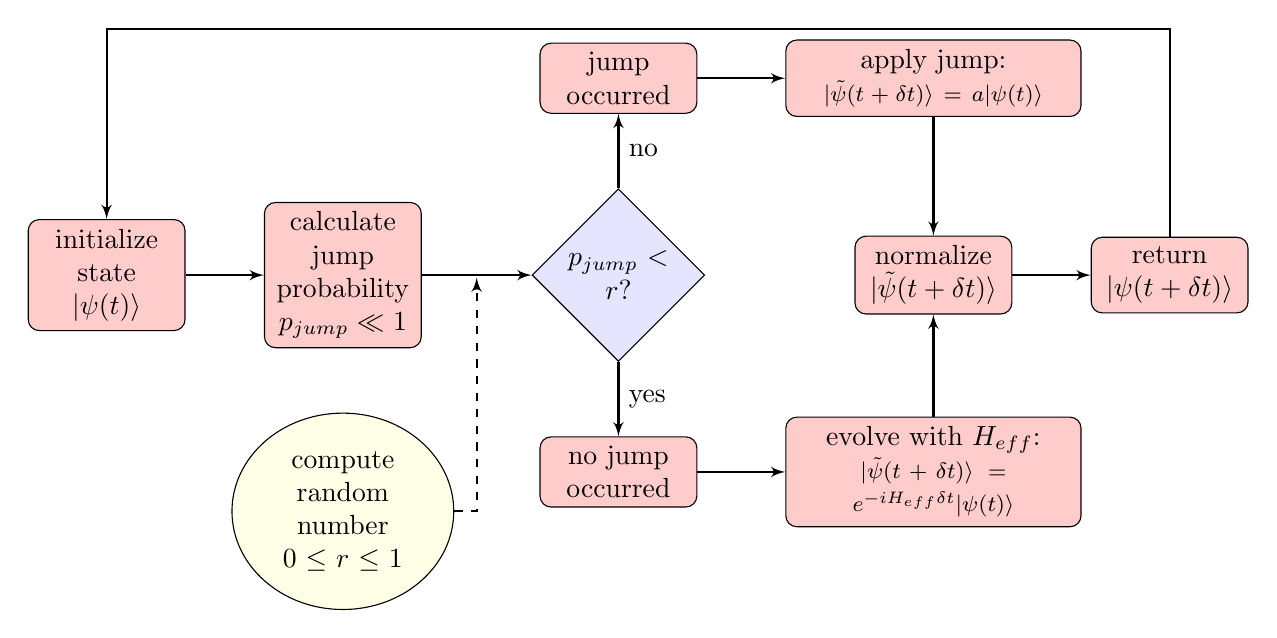
\begin{tikzpicture}[every text node part/.style={align=center}]

        % Place nodes

        \node [block] (init) {initialize state \\ $|\psi(t)\rangle$};
        \node [block, right of=init] (prob) {calculate jump probability \\
            $p_\text{jump}
        \ll 1$};
        \node [decision, right of=prob,node distance=3.5cm] (decide) {$p_\text{jump} < r$?};
        \node [block, below of=decide, node distance=2.5cm] 
                (no jump) {no jump occurred};
        \node [block, above of=decide, node distance=2.5cm] (jump) {jump
        occurred};
        \node [block, text width=10em, right of=no jump, node distance=4cm] (evolve) 
              {evolve with $H_\text{eff}$: \\ {\footnotesize
              $|\tilde{\psi}(t+\delta t)\rangle
              = e^{-iH_\text{eff} \delta t} |\psi(t)\rangle$}};
        \node [block, text width=10em, right of=jump, node distance=4cm] (apply jump) 
              {apply jump: \\ {\footnotesize$|\tilde{\psi}(t+\delta t)\rangle
              = a |\psi(t)\rangle$}};
        \node [block, right of=decide, node distance=4cm ] (normalize)
        {normalize $|\tilde{\psi}(t + \delta t) \rangle$};
        \node [block, right of=normalize, node distance=3cm] (return) {return $|\psi(t + \delta
        t)\rangle$};

        \node [cloud, below of=prob] (calc r) {compute random number \\ $0 \leq
        r \leq 1$};

        % Draw edges

        \path [line] (init) -- (prob);
        \path [line] (prob) -- node[midway, inner sep=0pt] (mid) {} (decide);
        \path [line] (decide) -- node[midway, right] {yes} (no jump);
        \path [line] (decide) -- node[midway, right] {no} (jump);
    
        \path [line, dashed] (calc r) -| (mid); 

        \path [line] (jump) -- (apply jump);
        \path [line] (no jump) -- (evolve);

        \path [line] (apply jump) -- (normalize);
        \path [line] (evolve) -- (normalize);

        \path [line] (normalize) -- (return);

        \path [line] (return.north) |- ([yshift=0.5em] jump.north) -|
        (init.north);
        

    \end{tikzpicture}
\end{document}
